\documentclass[a4 paper]{article}
\usepackage[inner=2.0cm,outer=2.0cm,top=2.5cm,bottom=2.5cm]{geometry}
\usepackage{setspace}
\usepackage{amsgen,amsmath,amstext,amsbsy,amsopn,tikz,amssymb}
\usepackage{booktabs}
\usepackage{framed}
\usepackage{diagbox}
\usepackage{tikz}
\usepackage{float}

% Symbols
\renewcommand{\epsilon}{\varepsilon}
\newcommand{\T}{\top}

% Linear algebra
\renewcommand{\vec}[1]{\boldsymbol{#1}}
\newcommand{\norm}[2][]{\lVert #2 \rVert _{#1}}

% Operator
\renewcommand{\ge}{\geqslant}
\renewcommand{\le}{\leqslant}
\newcommand{\vecdot}{\cdot}

\newcommand{\homework}[6]{
	\pagestyle{myheadings}
	\thispagestyle{plain}
	\newpage
	\setcounter{page}{1}
	\noindent
	\begin{center}
		\framebox{
			\vbox{\vspace{2mm}
				\hbox to 6.28in { {\bf Machine Learning \hfill {\small (#2)}} }
				\vspace{6mm}
				\hbox to 6.28in { {\Large \hfill #1  \hfill} }
				\vspace{6mm}
				\hbox to 6.28in { {\it Instructor: {\rm #3} \hfill Name: {\rm #5}, ID: {\rm #6}} }
				%\hbox to 6.28in { {\it TA: #4  \hfill #6}}
				\vspace{2mm}}
		}
	\end{center}
	\markboth{#5 -- #1}{#5 -- #1}
	\vspace*{4mm}
}

\newcounter{problem}[section]
\newcommand{\problem}[1]{~\newline\fbox{\textbf{Problem \refstepcounter{problem}\theproblem: #1}}\newline\newline}
\newcounter{subproblem}[problem]
\newcommand{\subproblem}{~\newline\textbf{(\refstepcounter{subproblem}\thesubproblem)}~}
\newenvironment{solution}{\newpage\setcounter{problem}{0}\begin{framed}\section*{Answer:}}{\vspace{15pt}\end{framed}}

%%%%%%%%%%%%%%%%%%%%%%%%%%%%%%%%%%%%%%%%%%%%%%%%%%%%%%%%%%%%%%%%%%%%%%%%%%%%%%%%%%%%%%%%%%%%%%%%%%%%%%%%%%%%
%   Please add your name and student ID to the {} below

\newcommand{\studentname}{Xu Danying}
\newcommand{\studentID}{58119213}

%%%%%%%%%%%%%%%%%%%%%%%%%%%%%%%%%%%%%%%%%%%%%%%%%%%%%%%%%%%%%%%%%%%%%%%%%%%%%%%%%%%%%%%%%%%%%%%%%%%%%%%%%%%%

\begin{document}
	\homework{Assignment \#4 (Neural Networks)}{Due: 20th June}{Beilun Wang}{}{\studentname}{\studentID}
	
	\section*{Problem Description:}
	
	\problem{Model selection and learning theory}
	
	\subproblem Let $X_i,\ i=1,2,\cdots,n$ be $n$ i.i.d observations from CDF $F(t)=P(X\le t)$. If we estimate the true CDF by empirical CDF which is
	\[\hat F_n(t)=\frac1n\sum_{i=1}^n\mathcal I(X_i\le t)\]
	where $\mathcal I(p)=1$ if statement $p$ is true, otherwise 0.
	
	Write down the expectation and variance of $\hat F_n(t)$. Then use Khinchin's law(i.e., the weak law of large numbers) to show that $\hat F_n(t)\xrightarrow P F(t)$.
	
	\subproblem Supoose we have a target variable $y$ and a vector of inputs $\vec x$, and the true model is $f(\vec x)$. If we assume that $y = f(\vec x) + \epsilon$ where $\epsilon$ is a Gaussian noise with $E(\epsilon) = 0$ and $Var(\epsilon) = \sigma_\epsilon^2$, we can derive an expression for the expected prediction error of a regression fit $\hat{f}(\vec x)$ at an point $\vec x = \vec x_0$, using squared-error loss:\[EPE(\vec x_0) = \sigma_\epsilon^2 + Bias^2(\hat f(\vec x_0)) + Var(\hat f(\vec x_0)).\]
	
	Now give training set $\vec X$ and the corresponding labels $\vec y$.
	
	(a) For a linear model fit $\hat{f_p}(\vec x) = \vec{x^\T\hat{\beta}}$, where the parameter vector $\hat{\vec\beta}$ with $p$ components is fit by least squares, write down the closed form solution of $\hat{\vec\beta}$. (\textit{Assume that $\vec X^\T \vec X$ is invertible.})
	
	If $\hat{\vec\beta}$ is fit by least squares using ridge regression with regularization parameter $\alpha$, we can get a model $\hat{f_\alpha}(\vec x)$. Also write down the closed form solution of $\hat{\vec{\beta}}_\alpha$.
	
	(b) For the linear model $\hat{f_p}(\vec x) = \vec{x^\T\hat{\beta}}$, write down the expression of EPE at $\vec x = \vec x_0$ using the solution $\hat{\vec\beta}$ in (a). (\textit{Assume only $y$ is random variable}).
	
	(c) For the model $\hat{f_\alpha}(\vec x) = \vec{x^\T\hat{\beta}_\alpha}$, write the down the expression of EPE at $\vec x = \vec x_0$ using the solution $\hat{\vec{\beta}}_\alpha$ in (a). (\textit{Assume only $y$ is random variable}).
	
	\subproblem Suppose we stack the outcomes $y_1,y_2,...y_N$ into a vector $\vec y$, and similarly for the predictions $\hat{\vec y}$. Then a linear fitting method is one for which we can write\[\hat{\vec y} = \vec{Sy},\] where $S$ is an $N\times N$ matrix depending on the input vectors $x_i$ but not on the $y_i$.\\
	Let $\hat{\vec f} = \vec{Sy}$ be a linear fitting of $\vec y$, and let ${\hat{\vec f}}^{-i}$ be the fitted function computed with $(\vec x_i, y_i)$ removed. If $S_{ii}$ is the $i$th diagonal element of $\vec S$, show that for $$\vec S = \vec X (\vec{X^\T X} + \lambda\vec\Omega)^{-1}\vec X^\T = \vec{XA^{-1}X^\T}(A\ is\ PSD)$$ the cross-validated residual can be written as\[y_i - {\hat f}^{-i}(\vec x_i) = \frac{y_i - \hat f (\vec x_i)}{1 - S_{ii}}\]
	(\textbf{Hint}: use a lemma $(\vec A - \vec{xx^\T})^{-1} = \vec A^{-1} + \frac{\vec {A^{-1}xx^\T\vec A^{-1}}}{1 - \vec{x^\T A^{-1}x}}$)
	
	\vspace{60pt}
	
	\problem{Neural Networks}
	
	Suppose that we apply neural networks on a problem which has boolean inputs $\vec x\in\{0,1\}^p$ and boolean output $y\in\{0,1\}$. The network structure example is showed as below. In this example we set $p=2$, single hidden layer with 2 neurons, activation function $\mathrm{ReLU}(u)=u\ \mathrm{if}\ u>0\ \mathrm{otherwise}\ 0$, and an additional threshold function(e.g., $f(v)=1$ if $v>0$, otherwise $f(v)=0$) for output layer.
	
	\begin{figure}[H]
		\centering
		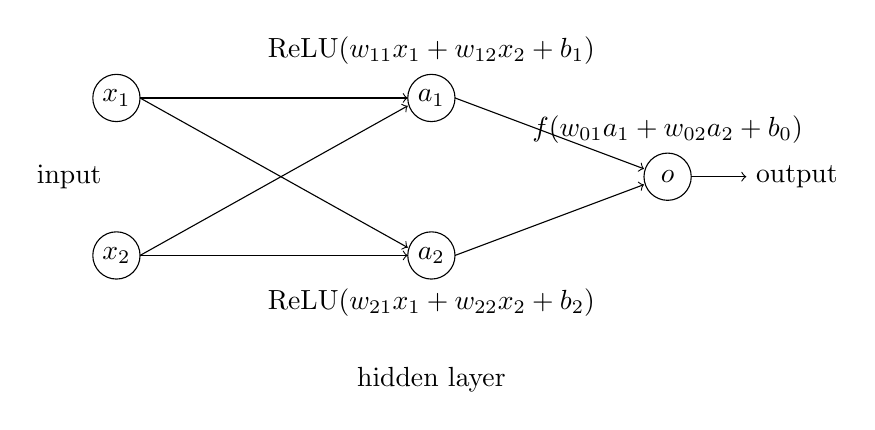
\begin{tikzpicture}
		\draw (0.4,0) node{input};
		\draw (1,1) circle [radius=0.3cm] node{$x_1$};
		\draw (1,-1) circle [radius=0.3cm] node{$x_2$};
		\draw (5,1) circle [radius=0.3cm] node[above=0.3cm]{ReLU($w_{11}x_1+w_{12}x_2+b_1$)} node{$a_1$};
		\draw (5,-1) circle [radius=0.3cm] node[below=0.3cm]{ReLU($w_{21}x_1+w_{22}x_2+b_2$)} node{$a_2$} node[below=1.3cm]{hidden layer};
		\draw (8,0) circle [radius=0.3cm] node[above=0.3cm]{$f(w_{01}a_1+w_{02}a_2+b_0)$} node{$o$};
		
		\draw [->] (1.3,1) -- (4.7,1);
		\draw [->] (1.3,-1) -- (4.7,-1);
		\draw [->] (1.3,1) -- (4.7,-0.9);
		\draw [->] (1.3,-1) -- (4.7,0.9);
		\draw [->] (5.3,1) -- (7.7,0.1);
		\draw [->] (5.3,-1) -- (7.7,-0.1);
		\draw [->] (8.3,0) -- (9,0) node[right]{output};
		\end{tikzpicture}
	\end{figure}
	
	
	\subproblem Using the structure and settings of neural network above, show that such a simple neural network could output the function $x_1$ XOR $x_2$(equals to 0 if $x_1=x_2$ and otherwise 1), which is impossible for linear models. State the values of parameters(i.e., $w_{ij}$ and $b_i$) you found.
	
	\subproblem Now we allow the number of neurons in the hidden layer to be more than 2 but finite. Retain the structure and other settings. Show that such a neural network with single hidden layer could output an arbitrary binary function $h:\ \{0,1\}^p\mapsto\{0,1\}$. You can apply threshold function after each neuron in the hidden layer.
	
	\begin{solution}
		%%%%%%%%%%%%%%%%%%%%%%%%%%%%%%%%%%%%%%%%%%%%%%%%%%%%%%%%%%%%%%%%%%%%%%%%%%%%%%%%%%%%%%%%%%%%%%%%%%%%%%%%%%%%%%%%%%%%%%%%%%%%%%
		
		% Please write down your answers in this environment.
		
		%%%%%%%%%%%%%%%%%%%%%%%%%%%%%%%%%%%%%%%%%%%%%%%%%%%%%%%%%%%%%%%%%%%%%%%%%%%%%%%%%%%%%%%%%%%%%%%%%%%%%%%%%%%%%%%%%%%%%%%%%%%%%%
		
		\problem{Model selection and learning theory}
		
		\subproblem
		Assume $y_i=\mathcal L(X_i\leq t)$, then $y_1,y_2,...,y_n$ are iid random variables.\\$\therefore E(y_i) = P(X_i\leq t) = F(t), E(y_i^2) = P(X_i\leq t) = F(t)\\\therefore D(y_i) = E(y_i^2)-{(Ey_i)}^2 = P(X_i\leq t) = F(t)\\\therefore \widehat F_n(t) = \frac1n\sum_{i=1}^ny_i\\\therefore E(\widehat F_n(t)) = \frac1n\times nF(t) = F(t),\\D(\widehat F_n(t)) = \frac1{n^2}nF(t)(1-F(t)) = \frac2nF(t)(1-F(t))$\\With Khinchin's law, $\widehat F_n(t)$ follows the theory for large numbers, so $\widehat F_n(t)\stackrel{P}{\longrightarrow}F(t)$.

		\subproblem
		
		(a)\\$\boldsymbol{\widehat\beta} = (\mathbf X^\top\mathbf X)^{-1}\mathbf X\mathbf y$,\\    $\widehat{\boldsymbol\beta}_{\alpha} = (\mathbf X^\top\mathbf X+\lambda\mathbf I)^{-1}\mathbf X\mathbf y$\\

		(b)$\\E(\widehat f_p(\mathbf x_0)) = E(\mathbf x_0^\top\widehat{\boldsymbol\beta})\\=E(\mathbf x_0^\top(\mathbf X^\top\mathbf X)^{-1}\mathbf X^\top\mathbf y)\\=\mathbf x_0^\top(\mathbf X^\top\mathbf X)^{-1}\mathbf X^\top Ey\\=\mathbf x_0^\top(\mathbf X^\top\mathbf X)^{-1}\mathbf X^\top E(f(\mathbf X)+\epsilon)\\=\mathbf x_0^\top(\mathbf X^\top\mathbf X)^{-1}\mathbf X^\top f(\mathbf X)$\\

$Bias(\widehat{f_p}(\mathbf x_0)) = E(f(\mathbf x_0)-E\widehat f_p(\mathbf x_0))\\=f(\mathbf x_0)-E(\widehat f(\mathbf x_0)\\=f(\mathbf x_0)-\mathbf x_0^\top(\mathbf X^\top\mathbf X)^{-1}\mathbf X^\top f(\mathbf X)$\\

$Var(\widehat{f_p}(\mathbf x_0)) =E(\widehat f_p(\mathbf x_0)-E(\widehat f_p(\mathbf x_0)))^2 \\=E(\mathbf x_0^\top(\mathbf X^\top\mathbf X)^{-1}\mathbf X^\top\mathbf y-\mathbf x_0^\top(\mathbf X^\top\mathbf X)^{-1}\mathbf X^\top f(\mathbf X))^2\\=E(\mathbf x_0^\top(\mathbf X^\top\mathbf X)^{-1}\mathbf X^\top (\mathbf y-f(\mathbf X)))^2\\=||\mathbf x_0^\top(\mathbf X^\top\mathbf X)^{-1}\mathbf X^\top ||^2\sigma_\epsilon^2$\\\\$\therefore EPE(\mathbf x_0) = \sigma_\epsilon^2+Bias^2(\widehat f_p(\mathbf x_0)+Var(\widehat f_p(\mathbf x_0))\\$


		(c)$\\E(\widehat f_\alpha(\mathbf x_0)) = \mathbf x_0^\top(\mathbf X^\top\mathbf X+\lambda\mathbf I)^{-1}\mathbf X^\top f(\mathbf X)\\Bias(\widehat f_\alpha(\mathbf x_0)) = f(\mathbf x_0)-\mathbf x_0^\top(\mathbf X^\top\mathbf X+\lambda\mathbf I)^{-1}\mathbf X^\top f(\mathbf X)\\Var(\widehat f_\alpha(\mathbf x_0))=||\mathbf x_0^\top(\mathbf X^\top\mathbf X+\lambda\mathbf I)^{-1}\mathbf X^\top||^2\sigma_\epsilon^2\\\therefore EPE(\mathbf x_0)=\sigma_\epsilon^2+Bias^2(\widehat f_\alpha(\mathbf x_0)+Var(\widehat f_\alpha(\mathbf x_0))$
		
		\subproblem
		$\\\mathbf S=\mathbf X(\mathbf X^\top\mathbf X+\lambda\Omega)^{-1}\mathbf X^\top = \mathbf X\mathbf A^{-1}\mathbf X^\top\\\therefore S_{ii}=\mathbf x_i\mathbf A^{-1}\mathbf x_i^\top,\mathbf x_i=(\mathbf X_{i1},\mathbf X_{i2},...,\mathbf X_{ip})\\\mathbf A = \mathbf X^\top\mathbf X+\lambda\Omega = (\mathbf X^{-i})^\top\mathbf X^{-i}+\mathbf x_i^\top\mathbf x_i+\lambda\Omega$\\According to the lemma,\\$((\mathbf X^{-i})^\top\mathbf X^{-i}+\lambda\Omega)^{-1}\\=(\mathbf A-\mathbf x_i^\top\mathbf x_i)^{-1}\\=\mathbf A^{-1} +\frac{\mathbf A^{-1}\mathbf x_i^\top\mathbf x_i\mathbf A^{-1}}{1-\mathbf x_i\mathbf A^{-1}\mathbf x_i^\top}\\=\mathbf A^{-1}+\frac{\mathbf A^{-1}\mathbf x_i^\top\mathbf x_i\mathbf A^{-1}}{1-S_{ii}}\\\therefore \widehat f(\mathbf x) = \mathbf S\mathbf y = \mathbf X\mathbf A^{-1}\mathbf X^\top\mathbf y\\\therefore\widehat f(\mathbf x_i) = \mathbf x_i\mathbf A^{-}\mathbf X^\top\mathbf y\\\because\mathbf X^\top\mathbf y = (\mathbf X^{-i})^\top\mathbf y^{-i}+\mathbf x_i^\top y_i\\\therefore(\mathbf X^{-i})^\top\mathbf y^{-i} = \mathbf X^\top\mathbf y-\mathbf x_i^\top y_i\\\therefore\widehat f^{-i}(\mathbf x_i) = \mathbf x_i((\mathbf X^{-i})^\top\mathbf X^{-i}+\lambda\Omega)^{-1}(\mathbf X^{-i})^\top\mathbf y\\=\mathbf x_i(\mathbf A^{-i}+\frac{\mathbf A^{-1}\mathbf x_i^\top\mathbf x_i\mathbf A^{-1}}{1-S_{ss}}^{-1}(\mathbf X^\top\mathbf y-\mathbf x_i^\top y_i)\\=\widehat f(\mathbf x_i)+\frac{S_{ii}\widehat f(\mathbf x_i)}{1-S_{ii}}-S_{ii}y_i-\frac{S_{ii}^2y_i}{1-S_{ii}}\\\therefore y_i-\widehat f^{-1}(\mathbf x_i) = y_i-\frac{\widehat f(\mathbf x_i)\S_{ii}y_i}{1-S_{ii}}\\=\frac{y_i-\widehat f(\mathbf x_i)}{1-S_{ii}}$
		\vspace{20pt}
		
		\problem{Neural Networks}
		
		\subproblem
		$\omega_{11}=-2,\omega_{12}=2,b_1=1;\omega_{21}=2,\omega_{22}=-2,b_2=1;\omega_{o1}=1,\omega_{o2}=1,b_o=-2$\\When $x_1=0,x_2=0,a_1=RELU(1)=1,a_2=RELU(1)=1,o=f(1+1-2)=0.$\\When $x_1=0,x_2=1,a_1=RELU(2+1)=3,a_2=RELU(-2+1)=0,o=f(3-2)=1.$\\When $x_1=1,x_2=0,a_1=RELU(-2+1)=0,a_2=RELU(2+1)=3,o=f(3-2)=1.$\\When $x_1=1,x_2=1,a_1=RELU(-2+2+1)=1,a_2=RELU(2-2+1)=1,o=f(1+1-2)=0.$\\
		\subproblem
		The operation "and", "or" and "negation" can be realized by using a perception. For any arbitrary binary function h, it is possible to list the corresponding truth table. In the truth table, for those values that equals to 1,add a nueron that dose "and" in the hidden layer to represent the line, and there are most $2^p$ nuerons in the hidden layers. Then, an "or" operation can be donein the output layer. In this way, we can realize a general bool operation through this neuron network.
	\end{solution}
	
\end{document} 
